\subsubsection{Modelo del mapa con Red de Petri} \mbox{} \vspace{10pt}

Como este trabajo tiene por objetivo el control, seguimiento del comportamiento y modelado de un sistema compuesto por una flota de robots donde cada uno tiene que seguir una trayectoria definida y calculada previamente utilizando el algoritmo A* determinando el camino más corto hacia su destino. Teniendo esto en mente es necesaria la implementación de un método para evitar los problemas inherentes en los sistemas multi-robot: las colisiones entre los robots y los bloqueos del sistema, haciendo que algunos robots no puedan terminar su trayectoria y por lo tanto entorpecer todo el sistema.

Al tener el conjunto de trayectorias definidas para cada robot, se modela el sistema y el mapa mediante el uso de Redes de Petri, que no son más que representaciones matemáticas con una representación gráfica de un sistema de eventos discretos. El entorno en el cual se mueven los robots se considera particionado el mapa en regiones (celdas) y cada región del mapa se modela como una plaza en la Red de Petri. Para evitar las colisiones entre los robots, se establecen regiones con capacidad finita (recursos), donde, no pueden pasar por ellas mas robots de los recursos definidos.

Si más de un robot desea pasar por la misma región en donde ya se encuentra posicionado un robot, el segundo debe esperar que la celda se libere y por lo tanto es necesario añadir lugares de espera. Estos lugares pueden conducir a bloqueos en la Red de Petri, ocasionando que los robots no lleguen a su destino. Los bloqueos se pueden caracterizar en la Red de Petri utilizando algunos elementos estructurales denominados sifones. Controlando que estos elementos no se vacíen, la red no se bloquea.

\begin{figure}[H]
   \centering
   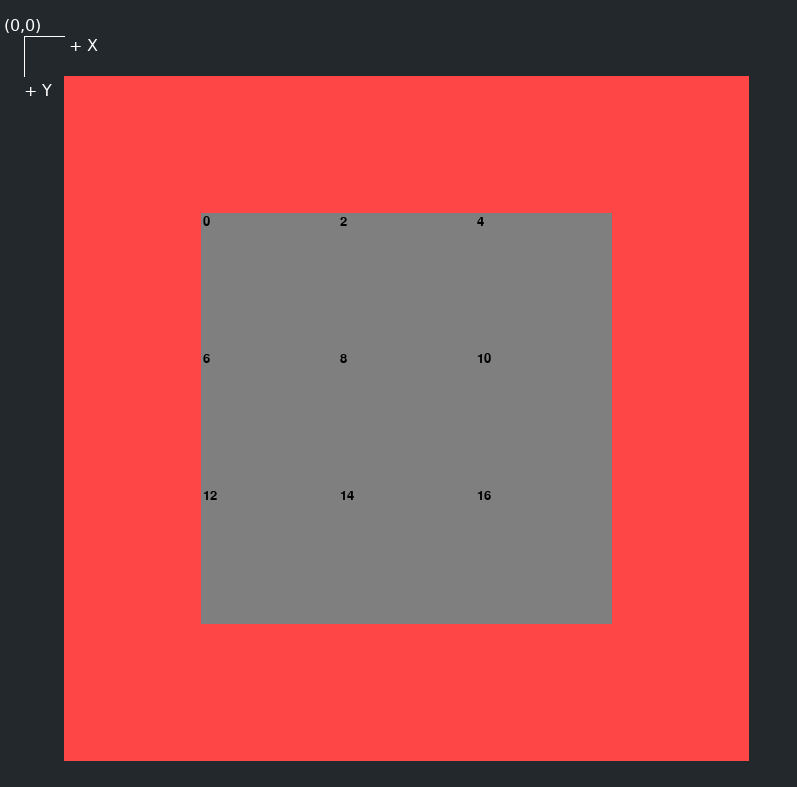
\includegraphics[width=0.6\linewidth]{images/mapa_py.png}
   \caption{Representación de un mapa en Python}
   \label{fig:mapa_py}
\end{figure}

La capacidad de las regiones, es decir, el número de robots que pueden estar simultáneamente en un lugar, se modela mediante los lugares de recursos, a los cuales se les asigna una marca (recurso), cuando el robot entra en una región específica y que se libera cuando el robot deja esa región.

Como ya se ha comentado la aplicación inmediata de los algoritmos implementados para este trabajo es la creación de una plataforma para el control de un sistema multi-robot con el objetivo de evitar colisiones entre los robots móviles. Sin embargo, se puede aplicar a cualquier sistema que sea modelable mediante redes de Petri. Por ello este proyecto tiene trascendencia en todas las áreas del control mediante sistemas de eventos discretos.

Antes de la implementación de uno de estos procesos, es muy importante moldearlo con un sistema discreto, comprobar su funcionamiento y corregirlo si hace falta. Las redes de Petri son una herramienta ampliamente utilizada cuando se trata de sistemas concurrentes, y como en cualquier otro sistema con recursos compartidos pueden aparecer bloqueos, así que este proyecto puede servir para resolver estos bloqueos haciendo el correcto uso de los recursos compartidos y gestionando de forma adecuada su utilización.

Un paso a realizar para obtener el modelo discreto del sistema multi-robot es dividir el mapa en regiones, ya que cada región del mapa se modelará como un lugar en el modelo de la red de Petri o como un nodo en el modelo de un autómata finito determinista. Para resolver el problema mencionado de dividir el mapa en regiones, se utiliza el método de la 'Descomposición en celdas'. Este método consiste en dividir las zonas sin obstáculos del plano mediante un cuadrado. Esto se puede claramente en la imagen anterior donde las celdas en color gris son las regiones disponibles o habitables por el robot mientras que las celdas rojas representan los límites del mapa.

Una vez descompuesto el mapa en regiones, queda calcular las trayectorias de cada robot para saber porque regiones ha de pasar para alcanzar de la forma más óptima el objetivo prefijado. Las trayectorias son obtenidas de forma automática a partir de algoritmos de cálculo de trayectorias individualmente para cada uno de los robots ignorando al resto de ellos utilizando algoritmos de búsqueda de caminos mínimos en grafos, o también pueden calcularse mediante algoritmos de planificación multi-robot ignorando las posibles colisiones entre los mismos utilizando programación matemática y modelos de tipo redes de Petri. En nuestro caso optamos por utilizar el algoritmo de A*, el cual busca el camino más corto para el robot hacía su destino último.

Si los dos robots individualmente siguen sus propias trayectorias, estos pueden colisionar (plazas ocupadas) ya que sus trayectorias pasan por esas regiones que tienen capacidad unitaria (un solo robot puede haber dentro de ellas en cualquier momento). Para evitar las posibles colisiones, se introducen modos de espera, es decir, se impone que por estas regiones no pueda pasar más de un robot al mismo tiempo, de modo que el segundo en llegar a esas regiones deberá esperar a que el primero salga de esa área.

Para sostener este concepto de regiones con capacidad limitada a las redes de Petri, se introducen lugares adicionales, a los que se les llama lugares de capacidades o de recursos compartidos. Estos lugares contienen inicialmente tantas marcas como capacidad tenga la región, en este caso se asignaran recursos con una marca a los lugares que corresponden a regiones con capacidad unitaria. Esta marca se utiliza para disparar la transición de entrada al lugar con capacidad limitada, y cuando el robot abandona esa zona, la transición de salida de ese lugar libera la marca para que vuelva a ser utilizada por el otro robot. Utilizando este concepto para todos los lugares con capacidad finita, la red quedaría como la siguiente.

\begin{figure}[H]
   \centering
   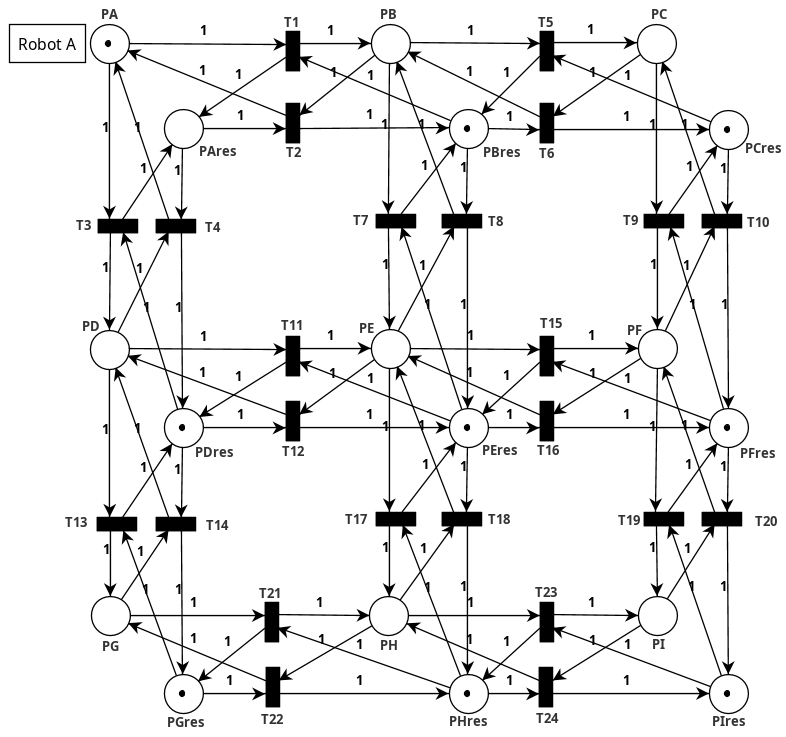
\includegraphics[width=0.8\linewidth]{images/rdp_no_grid.png}
   \caption{Representación del mapa en Python en una red de Petri}
   \label{fig:rdp_no_grid}
\end{figure}

Cabe destacar, que conforme va evolucionando el sistema y los robots se van moviendo de una región a otra, el marcado de la red va cambiando hasta que finalmente cuando un robot termina su trayectoria, la marca vuelve al lugar de reposo, sin embargo, el modelo de  red de Petri no podría volver a ser usado para supervisar el movimiento hasta que el robot sea colocado de nuevo en la posición de inicio del modelo.

Esta simple idea lo que hace es generar modos de espera de modo que nunca puedan coincidir en una región con capacidad restringida más de un robot. De modo que escogiendo correctamente estas regiones en las zonas donde las trayectorias de los robots coinciden, se pueden evitar las colisiones entre robots. Esto es debido a que los recursos compartidos producen modos de espera.

\paragraph{Transformación de un mapa a una red de Petri} \mbox{} \vspace{10pt}

Dentro del programa en Python existe una clase que se encarga de realizar esta transformación, el proceso consiste en definir la estructura que va a tener el mapa, es decir, cuáles van a ser sus espacios habitables y cuáles los límites. Entendiendo cómo límites a las paredes por fuera de la superficie de desplazamiento (su perímetro), y a los obstáculos que pueden existir dentro del mapa (paredes interiores, columnas, objetos, etc). Esto se hace en un archivo de texto que va a ser leído e interpretado por el algoritmo para luego ser convertido en una red de Petri.

\begin{figure}[H]
   \centering
   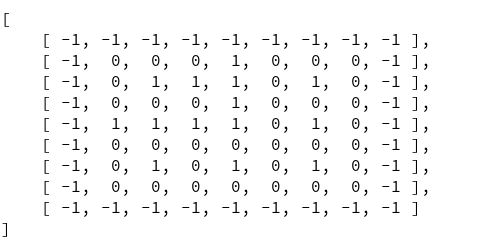
\includegraphics[width=0.6\linewidth]{images/map_definition.png}
   \caption{Matriz que define el mapa y sus elementos para el programa en Python}
   \label{fig:map_definition}
\end{figure}

El contenido del archivo que se muestra en la imagen anterior es el interpretado por el algoritmo y transformado. De este archivo se obtienen dos definiciones fundamentales para representar de forma correcta y suficiente a la red de Petri. Por un lado la matriz de incidencia, la cual nos describe la relación que existe entre las plazas y las transiciones de la red, es decir, como va a ser el movimiento de los tokens a medida que se disparen las transiciones, y por el otro lado el marcado inicial de la red, es decir, la distribución de los tokens en la red cuando todavía no se disparó ninguna transición. Cómo nosotros buscamos que la red cumpla ciertas condiciones para su adecuado comportamiento (por ejemplo no ser bloqueante), añadimos un lugar de recurso y un lugar de ocupación para celda habitable del mapa, es por ello que la imagen \ref{fig:rdp_no_grid} luce de esa manera.

Todo el proceso de transformación se encuentra descrito en la siguiente imagen, desde la lectura del archivo donde se define la estructura del mapa, pasando por su conversión a las matrices de incidencia y marcado, y por último en cómo el monitor toma esa red de Petri para decidir sobre el avance de los robots en el mapa.

\begin{figure}[H]
   \centering
   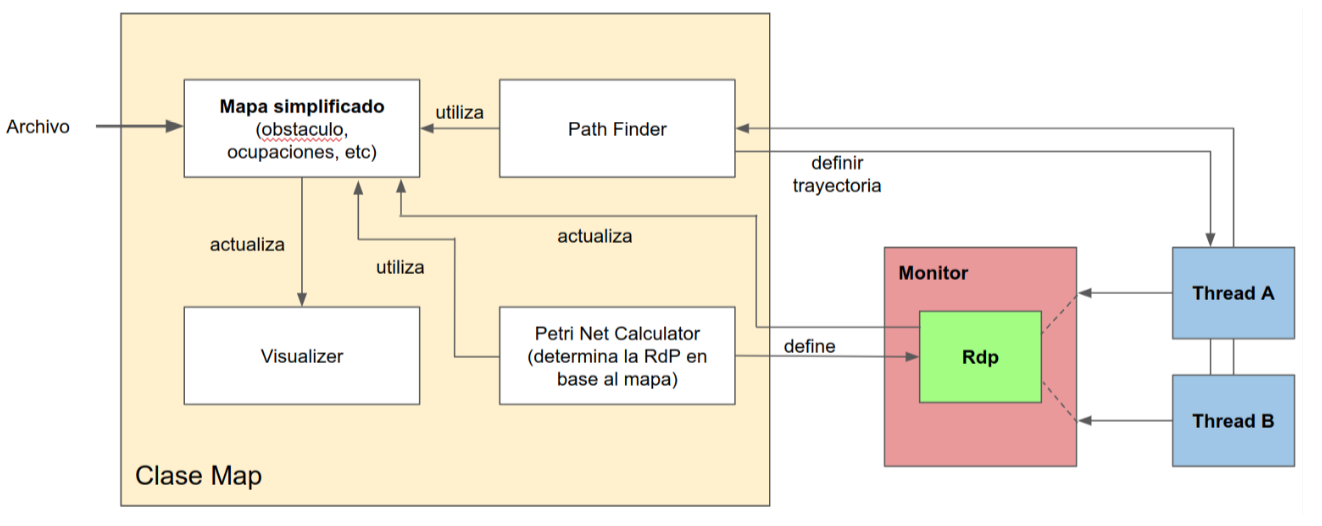
\includegraphics[width=1.0\linewidth]{images/mapa_to_rdp.png}
   \caption{Diagrama de alto nivel de la transformación de un mapa a una red de Petri}
   \label{fig:mapa_to_rdp}
\end{figure}